% !TEX root =./main.tex
\section{Block 2 : Time Gain Compensation - Csicsila}

    \subsection{Theory}
    As sound travels, it attenuates through geometric spreading.  As a result, the magnitude of the second reflected pulse is significantly lower. Therefore, the program must compensate to increase the magnitudes of the two pulses back to the original magnitude of 1. 
    The samples must first be converted into distance. This is easily accomplished using the following conversion.
    
    \begin{equation}
        r = \frac{\text{Sample Index}}{F_s} \cdot c_{\text{sound}}
        \label{eq:distanceTGC}
    \end{equation}
    
    

    For omni directional transducers the inverse-square law $(I \propto  \frac{1} {r^2} )$ dictates how the signal degraded with time. However, this signal was relatively directional and only degraded by $r$. In order to reduce the effects, the samples were multiplied by $1 + r$. Thus using a linear function to increase the magnitude of the first and second pulses.  


    \subsection{Analysis}

    \begin{figure}[H]
        \centering
        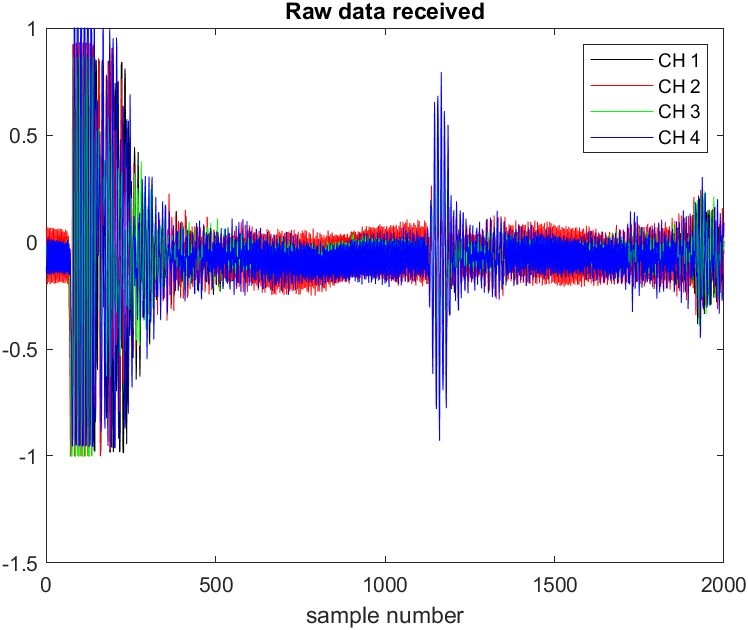
\includegraphics[width=0.5\linewidth]{figures/rawData.png}
        \caption{Raw Data}
        \label{fig:raw_data}
    \end{figure}

    Figure \ref{fig:raw_data} shows the initial signal detected. The goal of Block 2 is to boost the first and second pulses to a higher magnitude to increase clarity. As mentioned before, the pulses were boosted by multiplying the whole signal by distance traveled $r$.

    \begin{figure}[H]
        \centering
        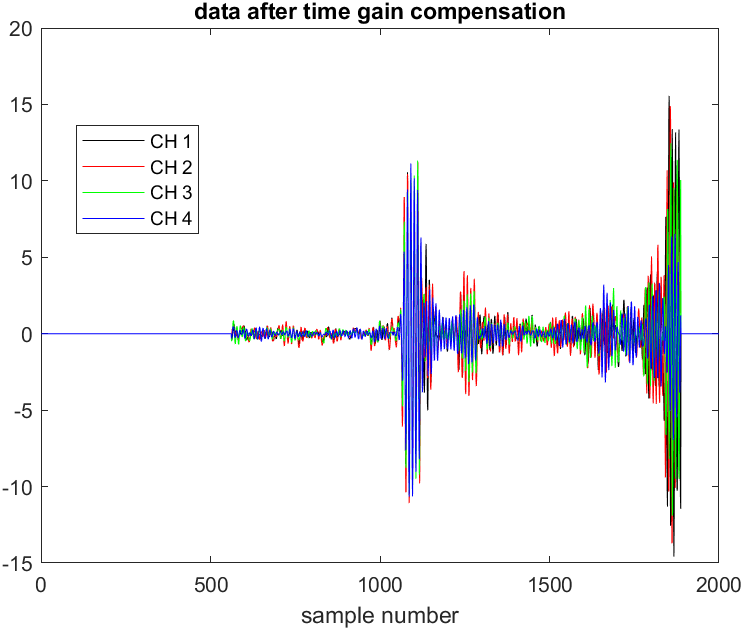
\includegraphics[width=0.5\linewidth]{figures/time_gain_1.png}
        \caption{Data after time gain compensation}
        \label{fig:time_gain1}
    \end{figure}

    
    Figure \ref{fig:time_gain1} shows the transformation after the attenuation. As seen, the first and second pulses are much closer in relative magnitude. Before, pulse 2 would be hidden due to its low magnitude. 

    \subsection{Performance}

    \begin{figure}[H]
        \centering
        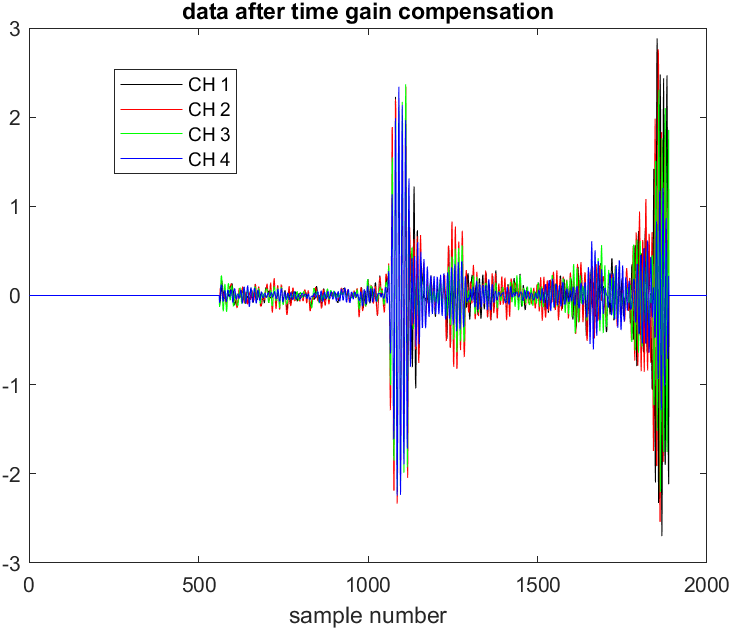
\includegraphics[width=0.5\linewidth]{figures/TGC_before.png}
        \caption{Data after time gain compensation provided}
        \label{fig:time_gain2}
    \end{figure}

    \begin{table}[H]
        \centering
        \begin{tabular}{cc}
            Function & Time ($\mu$s) \\ \hline
            Provided \code{.p} & $1435$\\
            Rewritten \code{.m} & $56.5$
        \end{tabular}
        \caption{Performance of TGC}
        \label{tab:TGCFunctionTime}
    \end{table}

    As seen in Table \ref{tab:TGCFunctionTime}, this implementation performed much quicker than the provided example. In addition it provided higher quality for the second pulse as seen in Figure \ref{fig:time_gain2}. The implementation was very simple, aiding its performance. The approach was creating an array for each channel and filling it with the values of the samples. Those values were then multiplied by $r$. The function timeGainCompensation then only had to multiply the data by the new array. This increased the speed by 184\%.
